\section{Specific requirements}

\subsection{External Interface Requirements}
Nothing here

\subsubsection{User Interfaces}
Nothing here

\subsubsection{Hardware Interfaces}
Nothing here

\subsubsection{Software Interfaces}
Nothing here

\subsubsection{Communication Interfaces}
Nothing here


\subsection{Functional Requirements}
\subsubsection{Use case diagrams}
\begin{enumerate}
    \item \textbf{Unregistered EV Driver}
          \begin{figure}[H]
              \centering
              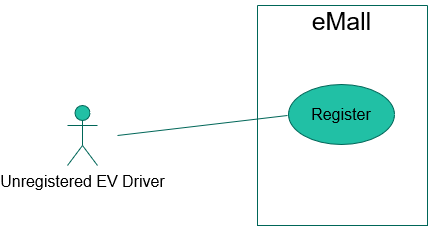
\includegraphics[scale=0.8]{src/use_case_diagram/driver_registration.png}
          \end{figure}
    \item \textbf{Unregistered CPO}
          \begin{figure}[H]
              \centering
              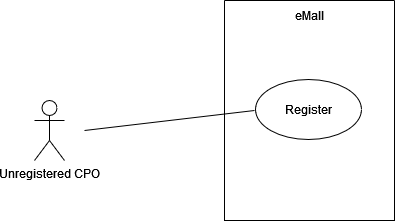
\includegraphics[scale=0.8]{src/use_case_diagram/cpo_registration.png}
          \end{figure}
    \item \textbf{CPO}
          \begin{figure}[H]
              \centering
              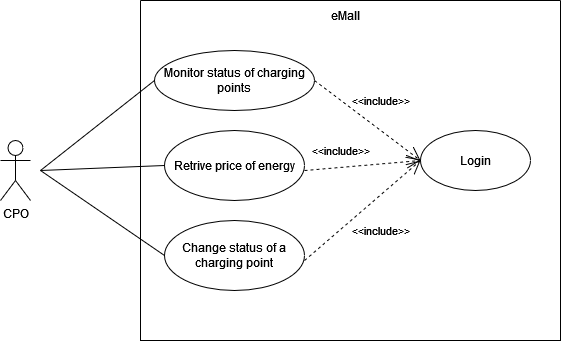
\includegraphics[scale=0.8]{src/use_case_diagram/cpo.png}
          \end{figure}
    \item \textbf{EV Driver}
\end{enumerate}
\subsubsection{CPOs}
\begin{table}[H]
    \begin{tabularx}{\textwidth}{cX}
        \toprule
        \textbf{R1}  & The system must allow unregistered operator to register an account and its EVSEs                                                  \\
        \textbf{R2}  & The system must allow making a special offer                                                                                      \\
        \textbf{R3}  & The system must allow monitoring the charging process to infer when the battery is full                                           \\
        \textbf{R4}  & The system must allow retrieving details on the amount of energy available in its EVSEs batteries                                 \\
        \textbf{R5}  & The system must allow retrieving details on the number of vehicle being charged and for each vehicle the amount of absorbed power \\
        \textbf{R6}  & The system must allow retrieving details on the charge time left for each connected vehicle                                       \\
        \textbf{R7}  & The system must allow retrieving details on active and historical reservations on its EVSEs                                       \\
        \textbf{R8}  & The system must allow acquiring information from the DSOs about the current price of energy                                       \\
        \textbf{R9}  & The system must allow deciding from which DSO to acquire energy from                                                              \\
        \textbf{R10} & The system must dynamically decide where to get energy for charging (electrical grid, battery or a mixture)                       \\ \bottomrule
    \end{tabularx}
\end{table}
\subsubsection{eMSP}
\begin{table}[H]
    \begin{tabularx}{\textwidth}{cX}
        \toprule
        \textbf{R11} & The system must allow unregistered users to register an account                                                     \\
        \textbf{R12} & The system must allow registered users to login                                                                     \\
        \textbf{R13} & The system must allow registered users to personalize his/her experience by providing information of his/her EV     \\
        \textbf{R14} & The system must allow users to search for EVSEs in the map                                                          \\
        \textbf{R15} & The system must show to the users EVSEs nearby his current position                                                 \\
        \textbf{R16} & The system must allow retrieving details on a given EVSE regarding connector types supported and cost of the charge \\
        \textbf{R17} & The system must allow booking of an EVSE for a certain time interval                                                \\
        \textbf{R18} & The system must allow booking of an EVSE if and only if it is free for the specified time interval                  \\
        \textbf{R19} & The system must notify users when the charging shift is about to start                                              \\
        \textbf{R20} & The system must allow users to start the charge                                                                     \\
        \textbf{R21} & The system must suggest users when to charge based on daily schedule, special offers and availability               \\
        \textbf{R22} & The system must allow users to monitor the charging status                                                          \\
        \textbf{R23} & The system must notify users when the charging process is completed                                                 \\
        \textbf{R24} & The system must allow users to pay for the charge                                                                   \\
        \textbf{R25} & The system must allow users to delete a reservation                                                                 \\
        \textbf{R26} & The system must allow users to view historical reservations                                                         \\ \bottomrule
    \end{tabularx}
\end{table}

\subsection{Performance Requirements}
Nothing here

\subsection{Design Constraints}
Nothing here

\subsubsection{Standards compliance}
Nothing here

\subsubsection{Hardware limitations}
Nothing here

\subsubsection{Any other constraint}
Nothing here


\subsection{Software System Attributes}
Nothing here

\subsubsection{Reliability}
Nothing here

\subsubsection{Availability}
Nothing here

\subsubsection{Security}
Nothing here

\subsubsection{Maintainability}
Nothing here

\subsubsection{Portability}
Nothing here
